\documentclass[sigconf]{acmart}

\usepackage{graphicx}
\usepackage{hyperref}
\usepackage{todonotes}

\usepackage{endfloat}
\renewcommand{\efloatseparator}{\mbox{}} % no new page between figures

\usepackage{booktabs} % For formal tables

\settopmatter{printacmref=false} % Removes citation information below abstract
\renewcommand\footnotetextcopyrightpermission[1]{} % removes footnote with conference information in first column
\pagestyle{plain} % removes running headers

\newcommand{\TODO}[1]{\todo[inline]{#1}}

\begin{document}
	\title{Why Deep Learning matters in IoT Data Analytics?}
	
	
	\author{Murali Cheruvu}
	\orcid{xxxx-xxxx-xxxx}
	\affiliation{%
		\institution{Indiana University}
		\streetaddress{3209 E 10th St}
		\city{Bloomington} 
		\state{Indiana} 
		\postcode{47408}
	}
	\email{mcheruvu@iu.edu}
	
	% The default list of authors is too long for headers}
	\renewcommand{\shortauthors}{M. Cheruvu}
	
	
	\begin{abstract}
		
	The Deep Learning is unique in all machine learning algorithms to analyze supervised and unsupervised datasets. Big Data challenges, such as high volumes, multi-dimensionality and feature engineering, are well addressed using Deep Learning algorithms. Deep Leaning, with Edge and distributed Mesh computing, is best suited to handle IoT Analytics from millions of sensors producing petabytes of time-series data.
			
	\end{abstract}
	
	\keywords{i523, hid306, IoT, Deep Learning, Big Data Analytics}
	
	\maketitle

	
	\section{Introduction}		

	Supervised machine learning algorithms: decision trees, linear regression, Support Vector Machines (SVMs), Naive Bayes, neural networks, etc. are popular for classification and regression problems by analyzing labeled training data. K-means clustering algorithms are good for unsupervised datasets to categorize based on the identified patterns in unlabeled data. While there are so many factors - nature of the domain, sample size of the dataset and number of attributes defining characteristics of the data - decide which machine learning algorithm works better, Deep Learning algorithms are, getting greater traction, addressing complex analytics tasks, including high-dimensionality and automatic creation of new features from existing complex hierarchical features, very well. 
		
	\section{Neural Networks}

	Neural Networks are inspired by human brain, the way they solve complex problems. {\em Perceptron}, the first generation neural network, created a simple mathematical model, mimicking neuron - the basic unit of the brain, by taking several binary inputs and produced single binary output. {\em Sigmoid Neuron} improved learning by giving some {\em weightage} to the input based on importance of the corresponding input to the output so that tiny changes in the output due to the minor adjustments in the input weights (or biases) can be measured effectively. Neural Network is, a {\em directed graph}, organized by layers and layers are created by number of interconnected nodes (or neurons). Every node in a layer is connected with all the nodes from the previous layer; there will no interaction of nodes within a layer. As shown in Figure (1), a typical Neural Network contains three layers: input (left), hidden (middle) and output (right) \cite{Goodfellow2016}. The middle layer is called {\em hidden} only because the nodes of this layer are neither an input nor an output but the actual processing happen in the hidden layer. As data passes through layer by layer, each node acts as an {\em activation function} to process the input. The performance of a Neural Network is measured using {\em cost or error function} and the dependent input {\em weight} variables. {\em Forward-propagation} and {\em back-propagation} are two techniques, neural network uses repeatedly until all the input variables are adjusted or calibrated to predict accurate output. During, forward-propagation, information moves in forward direction and passes through all the layers by applying certain weights to the input parameters. {\em Back-propagation} method minimizes the error in the {\em weights} by applying an algorithm called {\em gradient descent} at each iteration step. 	


	\begin{figure}
		\centering
		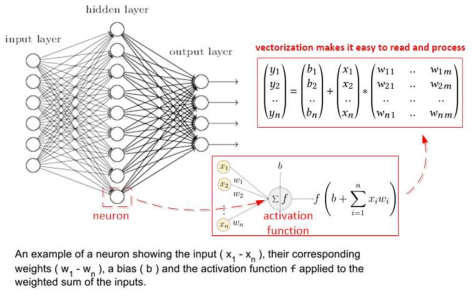
\includegraphics[width=0.5\textwidth]{images/neuralnetwork}
		\caption{Simple Neural Network \cite{Goodfellow2016, Gupta2017}.} \label{fig:figure1} 
	\end{figure}


	\section{Deep Learning}
	
	Deep Learning is an advanced neural network, with multiple hidden layers (thousands or even more deep), that can work well with supervised (labeled) and unsupervised (unlabeled) datasets. Applications, such as speech, image and behavior patterns, having complex relationships in large-set of attributes, are best suited for Deep Learning Neural Networks. Deep Learning vectorizes the input and converts it into output vector space by decomposing complex geometric and polynomial equations into a series of simple transformations. These transformations go through neuron activation functions at each layer parameterized by input weights. For it to be effective, the cost function of the neural network must guarantee two mathematical properties: {\em continuity} and {\em differentiability}.
	
	\begin{figure}
		\centering
		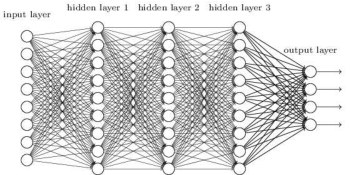
\includegraphics[width=0.5\textwidth]{images/deepnetwork}
		\caption{Deep Neural Network with three hidden layers \cite{Goodfellow2016}.} \label{fig:figure2} 
	\end{figure}

	\subsection{Feature Engineering}
	
	The dataset with too many dimensions, also known as attributes or features, create large sparsity and make it difficult to process. {\em Curse of dimensionality} is a scenario where the value added by the dimensions is much smaller in comparison to the processing cost. However, in certain applications, such as face recognition and patient electronic medical records, the complexity created by multiple dimensions might add value to the context. {\em Feature Engineering} is an exploratory analysis to identify the features that collectively contribute to better predictive modeling by removing irrelevant features and creating new features, using the training information to identify the patterns, from existing interrelated features \cite{JasonBrownlee2014}. {\em Principal Component Analysis} (PCA) is a technique to analyze the interdependency among the features and keep only the principal, most relevant, features with minimum loss in the model. With enough training, Deep Learning makes neurons learn new features themselves, in an unsupervised manner, from existing features distributed in several hidden layers. {\em Stacked Autoencoder} (AE) is, a Deep Belief Network algorithm, to create advanced predictive models for large datasets having thousands or even millions of dimensions, automatically, with complex hierarchical attributes in non-linear fashion for simpler computing. Though AE is sophisticated, it is very difficult to understand the algorithm logic and so unable to reuse the learnings from the modeling to other systems. 
		
	
	\subsection{Deep Neural Networks}
	
	{\em Convolutional Neural Network} (CNN) is a deep feedforward network, also called multilayer perceptron (MLP), consists of (1) convolutional layers - to identify the features using weights and biases, followed by (2) fully connected layers - where each neuron is connected from all the neurons of previous layers - to provide non-linearity, sub-sampling or max-pooling, performance and control data overfitting \cite{ChristopherOlah2014}. CNN is used in image and voice recognition applications by effectively using multiples copies of same neuron and reusing group of neurons in several places to make them {\em modular}. CNNs are constrained by {\em fixed-size} vectorized inputs and outputs. {\em Recursive Neural Network} (RNN) is, another type of Deep Learning, that uses same shared feature weights recursively for processing sequential data, emitted by sensors or the way spoken words are processed in natural language processing (NLP), to produce arbitrary size input and output vectors. RNN uses a technique called {\em loop}, where multiple copies of the same chunk of network (module), each passing a message to the next, to persist the information. Long Short Term Memory (LSTM) is an advanced RNN to learn and remember {\em longer} sequences by composing series of repeated modules of neural network and a concept called {\em cell state}, a memory unit, to memorize the learning by adding and removing information using {\em input}, {\em output} and {\em forget} gates, in a regularized fashion while data flows through the layers \cite{Olah2015}. The Convolutional and Recursive Neural Networks can complement each other to produce better and effective models where problem space has both - hierarchical features and temporal data. Deep Learning can also work well with related {\em Reinforcement Learning} algorithms where the focus is on how to maximize the learning based on rewards and punishments.	

	\begin{figure}
		\centering
		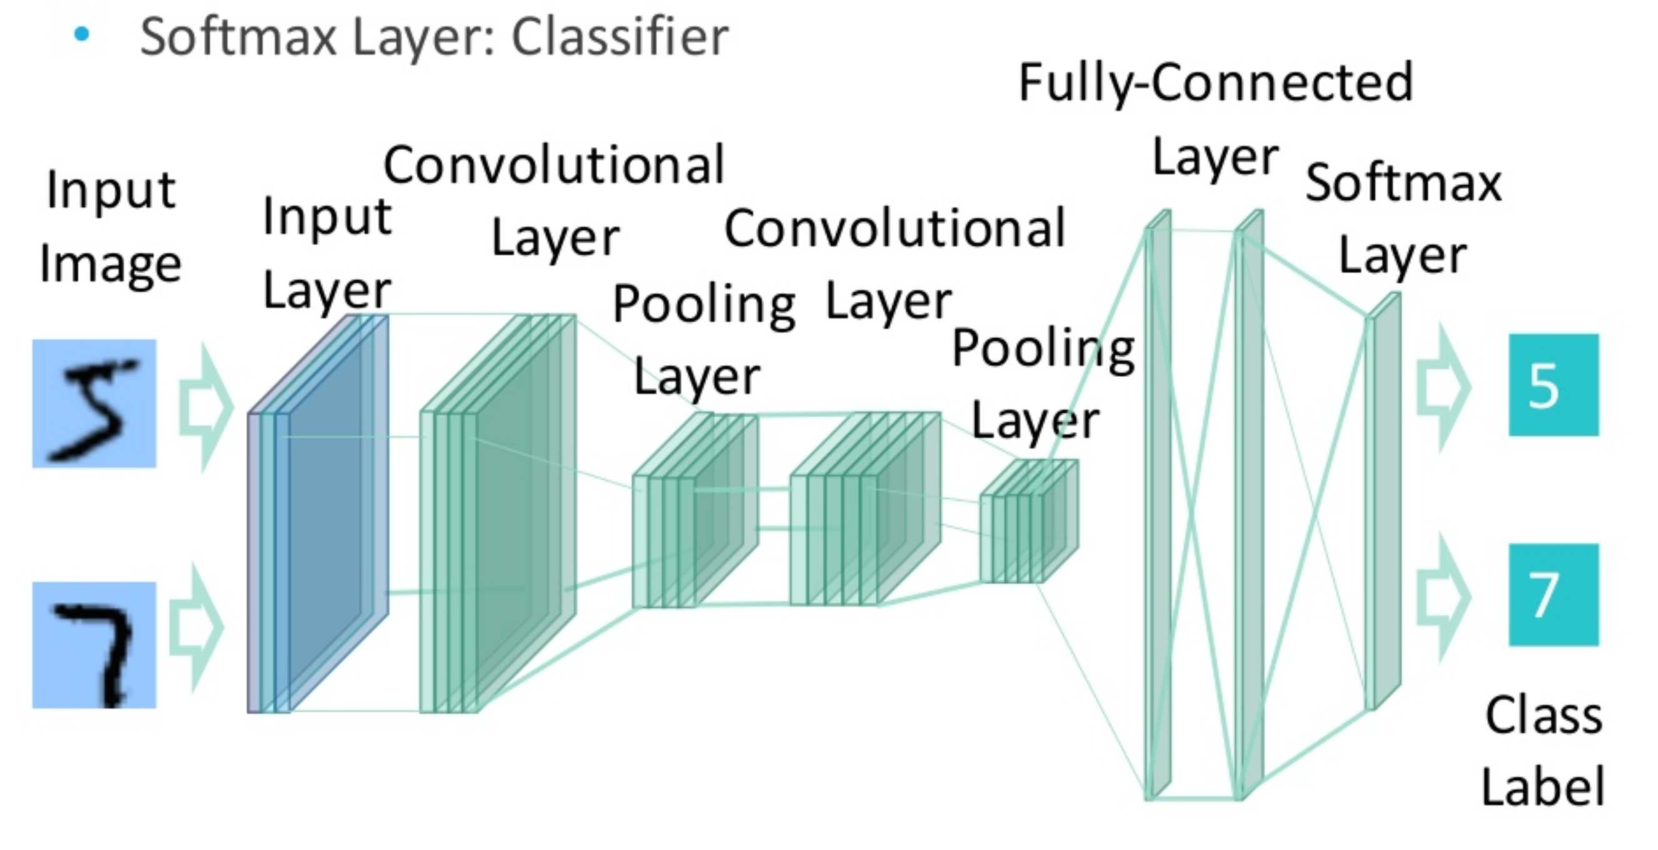
\includegraphics[width=0.5\textwidth]{images/cnn}
		\caption{Sample Convolutional Neural Network \cite{Chang2016}.} \label{fig:figure3} 
	\end{figure}

	\begin{figure}
		\centering
		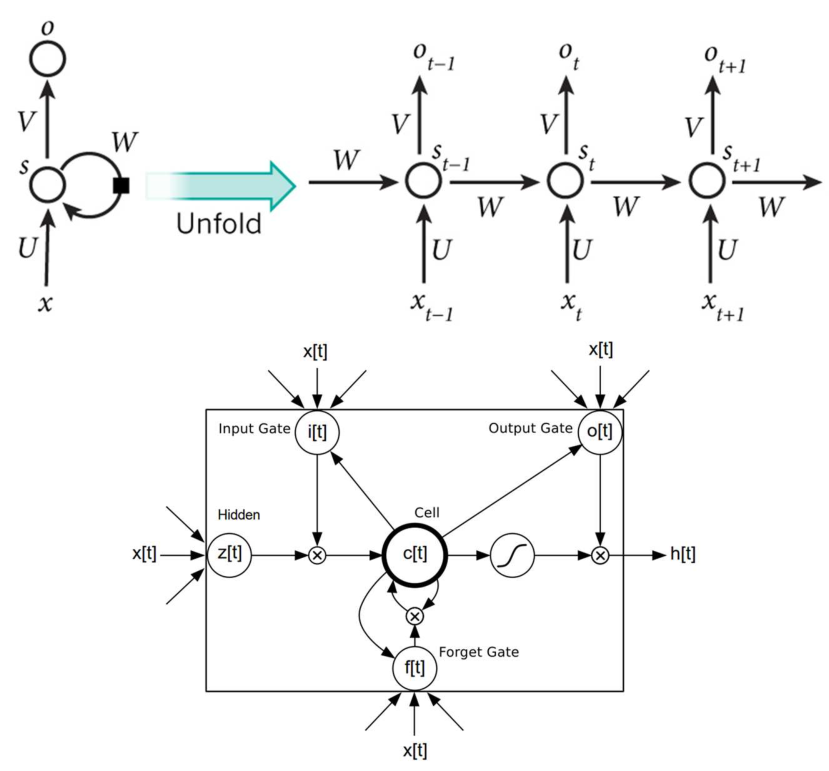
\includegraphics[width=0.5\textwidth]{images/rnn}
		\caption{Recursive Neural Network Loop and LSTM Cell State \cite{LeCun2015, Leonard2016}.} \label{fig:figure4} 
	\end{figure}

	
	\section{IoT Data Analytics}
	
	Internet of Things (IoT) is getting lots of traction, due to the massive volumes of data, making it {\em Big Data}; however, business needs to convert this data into {\em information} whether to monitor and control the devices or to analyze the sensor data for betterment. Time series data has non-stationary time aspects collected at certain intervals over a short period of time and correlate this sequence of data with past or future sequences. Stock prices and IoT sensor data are examples of time series data. {\em InfluxDB}, an open source time series database, is offering high write performance, data compaction through down-sampling and automatic deletion of expired old time series data, to address IoT data storage challenges \cite{Influx}.	
	
	
	\subsection{Complexity}
	
	Unique traits of IoT data, such as noise, high dimensionality and high streaming of time-series data in real-time, make it challenging to process using traditional machine learning algorithms \cite{Sampathkumar2016}. Autoregressive Moving Average Model (ARIMA), converts time-series from non-stationary into stationary, but only for short-time predictions. Deep Learning, using LSTM, can detect anomalies in the IoT Data and train time series data very well. Deep Learning algorithms involve complex mathematics - geometry, matrix algebra, differential calculus, statistics and probability, and intensive distributed computing to train the massive amounts of sensor data.
	
	\subsection{Scalability}
	
	Deep Learning, by design, allows parallel programming, as each module - with all the dependencies among neurons - can run independently and parallelly from other modules within the network. Using Graphics Process Unit (GPU), module networks can achieve parallel programming without needing much of Central Processing Unit (CPU) allocation. Though GPU is intended for graphical processing, it works efficiently to run thousands of small mathematical functions, such as matrix multiplications, in parallel. Cloud computing and Edge Analytics offer flexible scale out options, using virtualization and containerization, for distributed processing. Sophisticated algorithms and distributed computing make Deep Learning scale and perform well to process huge datasets. 
	
	\subsection{Case Study}
	
	Hewlett Packard (HP) Labs has given a presentation of their experiments to check how effectively Deep Learning algorithms can be applied for IoT Sensor Data Analytics. Sample data - vision, speech, text and sensor data such as signals, have been collected from scripted video and accelerometer from 52 subjects on average 20 minutes of activity recognition per subject - 12,000 measurements per minute per person with 16 classifications, such as walk to bed, enter bed, lie down, roll left, roll right and speak. They have analyzed and trained the sample data using various machine learning algorithms including Support Vector Machines (SVMs), Decision Trees and traditional Neural Networks; compared the results with Recurrent, Deep Learning, Neural Network. Deep Learning showed 95\% or more accuracy in various scenarios, performed much better than all the other algorithms, without sophisticated feature engineering. However, Deep Learning algorithms were slow and expensive for results to converge as the sample dataset is huge with lots of instances (10\textsuperscript{6}-10\textsuperscript{9}) and very large number of features ($>$10\textsuperscript{6}). They have concluded the presentation with scale-out hardware options using CPU/GPU clusters and futuristic Edge Analytics and distributed Mesh Computing alternatives for better scalability and performance \cite{Vassilieva2016}. 
			
	\section{Conclusion}		

	In contrast to traditional machine learning solutions, Deep Learning not only scales well with high volumes of input data but also facilitates in automatic decomposition of complex data representations of unsupervised and uncategorized data. Automatic discovery of new features, from convolutional or recurrent neural networks, makes Deep Learning predominant among all machine learning algorithms. It is very difficult to understand fuzzy and complex logic of Deep Learning, perhaps, more adoption helps getting better handle at them. Deep Learning algorithms need deep research in validating the process of advanced Big Data Analytics tasks, such as IoT sensor time-series data, semantic learning, scalability, data tagging and reliability of the predictive models without extreme generalization.  
	
	
	\begin{acks}		
	
		The author would like to thank Dr. Gregor von Laszewski and the Teaching Assistants for their support and valuable suggestions.
		
	\end{acks}

	\bibliographystyle{ACM-Reference-Format}
	\bibliography{report} 
	

	
\end{document}
